\documentclass[12pt,a4paper,fleqn,leqno]{article}
\usepackage{mathtext}
\usepackage{cmap}
\usepackage[utf8x]{inputenc}
\usepackage[russian]{babel}
\usepackage[T2A]{fontenc}
\usepackage{amsmath,amssymb,amsthm,amscd,amsfonts}
\usepackage{euscript}
\usepackage{relsize}
\usepackage{mathdots}
\usepackage{graphicx}
\usepackage{epstopdf}
\usepackage{caption2}
\usepackage{indentfirst}
\usepackage{fancyhdr}
\usepackage{sectsty}
\usepackage{titlesec}
\usepackage{sicpro_rus}
\usepackage{mathtext}%русские буквы в формулах

\usepackage[colorlinks, urlcolor=blue, pdfborder={0 0 0 [0 0]}]{hyperref}

\hyphenation{Struc-tu-red}
\hyphenation{Ran-do-mized}
\hyphenation{Ma-xi-mi-za-tion}
\DeclareMathOperator*{\argmax}{arg\,max}
\DeclareMathOperator*{\argmin}{arg\,min}
\DeclareMathOperator{\tr}{tr}
\providecommand*{\BibDash}{}

\def\rank{\mathop{\mathrm{rank}}}
\newtheorem{corollary}{Следствие}
\newtheorem{proposition}{Предложение}
\newtheorem{algorithm}{Алгоритм}
\newtheorem{lemma}{Лемма}

%new calligraphic font for subspaces
\usepackage{euscript}
\newcommand{\spA}{\EuScript{A}}
\newcommand{\spB}{\EuScript{B}}
\newcommand{\spC}{\EuScript{C}}
\newcommand{\spD}{\EuScript{D}}
\newcommand{\spE}{\EuScript{E}}
\newcommand{\spF}{\EuScript{F}}
\newcommand{\spG}{\EuScript{G}}
\newcommand{\spH}{\EuScript{H}}
\newcommand{\spI}{\EuScript{I}}
\newcommand{\spJ}{\EuScript{J}}
\newcommand{\spK}{\EuScript{K}}
\newcommand{\spL}{\EuScript{L}}
\newcommand{\spM}{\EuScript{M}}
\newcommand{\spN}{\EuScript{N}}
\newcommand{\spO}{\EuScript{O}}
\newcommand{\spP}{\EuScript{P}}
\newcommand{\spQ}{\EuScript{Q}}
\newcommand{\spR}{\EuScript{R}}
\newcommand{\spS}{\EuScript{S}}
\newcommand{\spT}{\EuScript{T}}
\newcommand{\spU}{\EuScript{U}}
\newcommand{\spV}{\EuScript{V}}
\newcommand{\spW}{\EuScript{W}}
\newcommand{\spX}{\EuScript{X}}
\newcommand{\spY}{\EuScript{Y}}
\newcommand{\spZ}{\EuScript{Z}}

%font for text indices like transposition X^\mathrm{T}
\newcommand{\rmA}{\mathrm{A}}
\newcommand{\rmB}{\mathrm{B}}
\newcommand{\rmC}{\mathrm{C}}
\newcommand{\rmD}{\mathrm{D}}
\newcommand{\rmE}{\mathrm{E}}
\newcommand{\rmF}{\mathrm{F}}
\newcommand{\rmG}{\mathrm{G}}
\newcommand{\rmH}{\mathrm{H}}
\newcommand{\rmI}{\mathrm{I}}
\newcommand{\rmJ}{\mathrm{J}}
\newcommand{\rmK}{\mathrm{K}}
\newcommand{\rmL}{\mathrm{L}}
\newcommand{\rmM}{\mathrm{M}}
\newcommand{\rmN}{\mathrm{N}}
\newcommand{\rmO}{\mathrm{O}}
\newcommand{\rmP}{\mathrm{P}}
\newcommand{\rmQ}{\mathrm{Q}}
\newcommand{\rmR}{\mathrm{R}}
\newcommand{\rmS}{\mathrm{S}}
\newcommand{\rmT}{\mathrm{T}}
\newcommand{\rmU}{\mathrm{U}}
\newcommand{\rmV}{\mathrm{V}}
\newcommand{\rmW}{\mathrm{W}}
\newcommand{\rmX}{\mathrm{X}}
\newcommand{\rmY}{\mathrm{Y}}
\newcommand{\rmZ}{\mathrm{Z}}

%tt font for time series
\newcommand{\tsA}{\mathbb{A}}
\newcommand{\tsB}{\mathbb{B}}
\newcommand{\tsC}{\mathbb{C}}
\newcommand{\tsD}{\mathbb{D}}
\newcommand{\tsE}{\mathbb{E}}
\newcommand{\tsF}{\mathbb{F}}
\newcommand{\tsG}{\mathbb{G}}
\newcommand{\tsH}{\mathbb{H}}
\newcommand{\tsI}{\mathbb{I}}
\newcommand{\tsJ}{\mathbb{J}}
\newcommand{\tsK}{\mathbb{K}}
\newcommand{\tsL}{\mathbb{L}}
\newcommand{\tsM}{\mathbb{M}}
\newcommand{\tsN}{\mathbb{N}}
\newcommand{\tsO}{\mathbb{O}}
\newcommand{\tsP}{\mathbb{P}}
\newcommand{\tsQ}{\mathbb{Q}}
\newcommand{\tsR}{\mathbb{R}}
\newcommand{\tsS}{\mathbb{S}}
\newcommand{\tsT}{\mathbb{T}}
\newcommand{\tsU}{\mathbb{U}}
\newcommand{\tsV}{\mathbb{V}}
\newcommand{\tsW}{\mathbb{W}}
\newcommand{\tsX}{\mathbb{X}}
\newcommand{\tsY}{\mathbb{Y}}
\newcommand{\tsZ}{\mathbb{Z}}

%bf font for matrices
\newcommand{\bfA}{\mathbf{A}}
\newcommand{\bfB}{\mathbf{B}}
\newcommand{\bfC}{\mathbf{C}}
\newcommand{\bfD}{\mathbf{D}}
\newcommand{\bfE}{\mathbf{E}}
\newcommand{\bfF}{\mathbf{F}}
\newcommand{\bfG}{\mathbf{G}}
\newcommand{\bfH}{\mathbf{H}}
\newcommand{\bfI}{\mathbf{I}}
\newcommand{\bfJ}{\mathbf{J}}
\newcommand{\bfK}{\mathbf{K}}
\newcommand{\bfL}{\mathbf{L}}
\newcommand{\bfM}{\mathbf{M}}
\newcommand{\bfN}{\mathbf{N}}
\newcommand{\bfO}{\mathbf{O}}
\newcommand{\bfP}{\mathbf{P}}
\newcommand{\bfQ}{\mathbf{Q}}
\newcommand{\bfR}{\mathbf{R}}
\newcommand{\bfS}{\mathbf{S}}
\newcommand{\bfT}{\mathbf{T}}
\newcommand{\bfU}{\mathbf{U}}
\newcommand{\bfV}{\mathbf{V}}
\newcommand{\bfW}{\mathbf{W}}
\newcommand{\bfX}{\mathbf{X}}
\newcommand{\bfY}{\mathbf{Y}}
\newcommand{\bfZ}{\mathbf{Z}}

%bf font for hilbert space
\newcommand{\bfa}{\mathbf{a}}
\newcommand{\bfb}{\mathbf{b}}
\newcommand{\bfc}{\mathbf{c}}
\newcommand{\bfd}{\mathbf{d}}
\newcommand{\bfe}{\mathbf{e}}
\newcommand{\bff}{\mathbf{f}}
\newcommand{\bfg}{\mathbf{g}}
\newcommand{\bfh}{\mathbf{h}}
\newcommand{\bfi}{\mathbf{i}}
\newcommand{\bfj}{\mathbf{j}}
\newcommand{\bfk}{\mathbf{k}}
\newcommand{\bfl}{\mathbf{l}}
\newcommand{\bfm}{\mathbf{m}}
\newcommand{\bfn}{\mathbf{n}}
\newcommand{\bfo}{\mathbf{o}}
\newcommand{\bfp}{\mathbf{p}}
\newcommand{\bfq}{\mathbf{q}}
\newcommand{\bfr}{\mathbf{r}}
\newcommand{\bfs}{\mathbf{s}}
\newcommand{\bft}{\mathbf{t}}
\newcommand{\bfu}{\mathbf{u}}
\newcommand{\bfv}{\mathbf{v}}
\newcommand{\bfw}{\mathbf{w}}
\newcommand{\bfx}{\mathbf{x}}
\newcommand{\bfy}{\mathbf{y}}
\newcommand{\bfz}{\mathbf{z}}

%bb font for standard spaces and expectation
\newcommand{\bbA}{\mathbb{A}}
\newcommand{\bbB}{\mathbb{B}}
\newcommand{\bbC}{\mathbb{C}}
\newcommand{\bbD}{\mathbb{D}}
\newcommand{\bbE}{\mathbb{E}}
\newcommand{\bbF}{\mathbb{F}}
\newcommand{\bbG}{\mathbb{G}}
\newcommand{\bbH}{\mathbb{H}}
\newcommand{\bbI}{\mathbb{I}}
\newcommand{\bbJ}{\mathbb{J}}
\newcommand{\bbK}{\mathbb{K}}
\newcommand{\bbL}{\mathbb{L}}
\newcommand{\bbM}{\mathbb{M}}
\newcommand{\bbN}{\mathbb{N}}
\newcommand{\bbO}{\mathbb{O}}
\newcommand{\bbP}{\mathbb{P}}
\newcommand{\bbQ}{\mathbb{Q}}
\newcommand{\bbR}{\mathbb{R}}
\newcommand{\bbS}{\mathbb{S}}
\newcommand{\bbT}{\mathbb{T}}
\newcommand{\bbU}{\mathbb{U}}
\newcommand{\bbV}{\mathbb{V}}
\newcommand{\bbW}{\mathbb{W}}
\newcommand{\bbX}{\mathbb{X}}
\newcommand{\bbY}{\mathbb{Y}}
\newcommand{\bbZ}{\mathbb{Z}}

%got font for any case
\newcommand{\gA}{\mathfrak{A}}
\newcommand{\gB}{\mathfrak{B}}
\newcommand{\gC}{\mathfrak{C}}
\newcommand{\gD}{\mathfrak{D}}
\newcommand{\gE}{\mathfrak{E}}
\newcommand{\gF}{\mathfrak{F}}
\newcommand{\gG}{\mathfrak{G}}
\newcommand{\gH}{\mathfrak{H}}
\newcommand{\gI}{\mathfrak{I}}
\newcommand{\gJ}{\mathfrak{J}}
\newcommand{\gK}{\mathfrak{K}}
\newcommand{\gL}{\mathfrak{L}}
\newcommand{\gM}{\mathfrak{M}}
\newcommand{\gN}{\mathfrak{N}}
\newcommand{\gO}{\mathfrak{O}}
\newcommand{\gP}{\mathfrak{P}}
\newcommand{\gQ}{\mathfrak{Q}}
\newcommand{\gR}{\mathfrak{R}}
\newcommand{\gS}{\mathfrak{S}}
\newcommand{\gT}{\mathfrak{T}}
\newcommand{\gU}{\mathfrak{U}}
\newcommand{\gV}{\mathfrak{V}}
\newcommand{\gW}{\mathfrak{W}}
\newcommand{\gX}{\mathfrak{X}}
\newcommand{\gY}{\mathfrak{Y}}
\newcommand{\gZ}{\mathfrak{Z}}

%old calligraphic font
\newcommand{\calA}{\mathcal{A}}
\newcommand{\calB}{\mathcal{B}}
\newcommand{\calC}{\mathcal{C}}
\newcommand{\calD}{\mathcal{D}}
\newcommand{\calE}{\mathcal{E}}
\newcommand{\calF}{\mathcal{F}}
\newcommand{\calG}{\mathcal{G}}
\newcommand{\calH}{\mathcal{H}}
\newcommand{\calI}{\mathcal{I}}
\newcommand{\calJ}{\mathcal{J}}
\newcommand{\calK}{\mathcal{K}}
\newcommand{\calL}{\mathcal{L}}
\newcommand{\calM}{\mathcal{M}}
\newcommand{\calN}{\mathcal{N}}
\newcommand{\calO}{\mathcal{O}}
\newcommand{\calP}{\mathcal{P}}
\newcommand{\calQ}{\mathcal{Q}}
\newcommand{\calR}{\mathcal{R}}
\newcommand{\calS}{\mathcal{S}}
\newcommand{\calT}{\mathcal{T}}
\newcommand{\calU}{\mathcal{U}}
\newcommand{\calV}{\mathcal{V}}
\newcommand{\calW}{\mathcal{W}}
\newcommand{\calX}{\mathcal{X}}
\newcommand{\calY}{\mathcal{Y}}
\newcommand{\calZ}{\mathcal{Z}}

%sf font for transposition and spaces like R
\newcommand{\sfA}{\mathsf{A}}
\newcommand{\sfB}{\mathsf{B}}
\newcommand{\sfC}{\mathsf{C}}
\newcommand{\sfD}{\mathsf{D}}
\newcommand{\sfE}{\mathsf{E}}
\newcommand{\sfF}{\mathsf{F}}
\newcommand{\sfG}{\mathsf{G}}
\newcommand{\sfH}{\mathsf{H}}
\newcommand{\sfI}{\mathsf{I}}
\newcommand{\sfJ}{\mathsf{J}}
\newcommand{\sfK}{\mathsf{K}}
\newcommand{\sfL}{\mathsf{L}}
\newcommand{\sfM}{\mathsf{M}}
\newcommand{\sfN}{\mathsf{N}}
\newcommand{\sfO}{\mathsf{O}}
\newcommand{\sfP}{\mathsf{P}}
\newcommand{\sfQ}{\mathsf{Q}}
\newcommand{\sfR}{\mathsf{R}}
\newcommand{\sfS}{\mathsf{S}}
\newcommand{\sfT}{\mathsf{T}}
\newcommand{\sfU}{\mathsf{U}}
\newcommand{\sfV}{\mathsf{V}}
\newcommand{\sfW}{\mathsf{W}}
\newcommand{\sfX}{\mathsf{X}}
\newcommand{\sfY}{\mathsf{Y}}
\newcommand{\sfZ}{\mathsf{Z}}

\newcommand{\bt}{\begin{theorem}}
\newcommand{\et}{\end{theorem}}
\newcommand{\bl}{\begin{lemma}}
\newcommand{\el}{\end{lemma}}
\newcommand{\bp}{\begin{proposition}}
\newcommand{\ep}{\end{proposition}}
\newcommand{\bc}{\begin{corollary}}
\newcommand{\ec}{\end{corollary}}

\newcommand{\bd}{\begin{definition}\rm}
\newcommand{\ed}{\end{definition}}
\newcommand{\bex}{\begin{example}\rm}
\newcommand{\eex}{\end{example}}
\newcommand{\br}{\begin{remark}\rm}
\newcommand{\er}{\end{remark}}

\newcommand{\btbh}{\begin{table}[!ht]}
\newcommand{\etb}{\end{table}}
\newcommand{\bfgh}{\begin{figure}[!ht]}
\newcommand{\efg}{\end{figure}}

\newcommand{\bea}{\begin{eqnarray*}}
\newcommand{\eea}{\end{eqnarray*}}
\newcommand{\be}{\begin{eqnarray}}
\newcommand{\ee}{\end{eqnarray}}
%
\newcommand{\intl}{\int\limits}
\newcommand{\suml}{\sum\limits}
\newcommand{\liml}{\lim\limits}
\newcommand{\prodl}{\prod\limits}
\newcommand{\minl}{\min\limits}
\newcommand{\maxl}{\max\limits}
\newcommand{\supl}{\sup\limits}
%
\newcommand{\ve}{\varepsilon}
\newcommand{\vphi}{\varphi}
\newcommand{\ovl}{\overline}
\newcommand{\lm}{\lambda}
\def\wtilde{\widetilde}
\def\what{\widehat}

\newcommand{\ra}{\rightarrow}
\newcommand{\towith}[1]{\mathrel{\mathop{\longrightarrow}_{#1}}}

\def\bproof{\textbf{Proof.\ }}
\def\eproof{\hfill$\Box$\smallskip}

\def\spaceN{\mathsf{N}}
\def\spaceZ{\mathsf{Z}}
\def\spaceR{\mathsf{R}}
\def\spaceC{\mathsf{C}} %is not used?
\newcommand\Expect{\mathsf{E}}
%\newcommand\Variance{\mathsf{D}}

\newcommand{\bfw}{\mathbf{w}}

\def\last#1{{\underline{#1}}}
\def\llast#1{\underline{\underline{#1}}}
\def\first#1{{\mathstrut\overline{#1}}}
\def\ffirst#1{\mathstrut\overline{\mathstrut\overline{#1}}}
\def\overo#1{\overset{_\mathrm{o}}{#1}}
\newcommand{\ontop}[2]{\genfrac{}{}{0pt}{0}{#1}{#2}}
\def\bfpi{\mbox{\boldmath{$\pi$}}}
\def\bfmu{\mbox{\boldmath{$\mu$}}}
\def\bfPi{\mbox{\boldmath{$\Pi$}}}
\def\bfcR{\mbox{\boldmath{$\cR$}}}

\def\mmod{\mathop{\mathrm{mod}}}
\def\sspan{\mathop{\mathrm{span}}}
\def\rank{\mathop{\mathrm{rank}}}
\def\dist{\mathop{\mathrm{dist}}}

\newcommand{\reverse}{\mathop{\mathrm{rev}}}
\newcommand{\Arg}{\mathop\mathrm{Arg}}
\newcommand{\meas}{\mathop{\mathrm{meas}}}

\newcommand{\colspace}{\mathop{\mathrm{colspace}}}
\newcommand{\rowspace}{\mathop{\mathrm{rowspace}}}


\makeatletter
\def\adots{\mathinner{\mkern2mu\raise\p@\hbox{.}
\mkern2mu\raise4\p@\hbox{.}\mkern1mu
\raise7\p@\vbox{\kern7\p@\hbox{.}}\mkern1mu}}
\newcommand{\l@abcd}[2]{\hbox to\textwidth{#1\dotfill #2}}
\makeatother

\def\func{\mathop\mathrm}

% Some new definitions
\newcommand{\defeq}{\stackrel{def}{=}}
\newcommand{\frob}{\calF}
\def\trajmat#1{\calT_{\mathrm{#1}}}

\def\unit{\mathfrak{i}}



\sectionfont{\centering}

\subsectionfont{\centering}
\subsubsectionfont{\normalsize}
\setcounter{page}{1}


\author{Nikita Zvonarev}
\title{Iterative algorithms for Weighted Finite Rank Time Series  Approximation}
\begin{document}
\noindent УДК 519.246.8+519.254

\begin{center}{
\fontsize{18pt}{23pt}\selectfont\bf%
  \MakeUppercase{
 Iterative algorithms for Weighted Finite Rank Time Series Approximation
}}
\end{center}

\begin{center}{\bpv\bmv {Н.К.~Звонарев}\\
\footnotesize\it Санкт-Петербургский государственный университет,\\
Математико-механический факультет
\\
\rm
Россия, 198504, Санкт-Петербург, Петродворец, Университетский пр., 28\\
E-mail: \textcolor {blue}{\underline{nikitazvonarev@gmail.com}}}
\end{center}
\begin{center}{\bpv {Н.Э.~Голяндина}\\
\footnotesize\it Санкт-Петербургский государственный университет,\\
Математико-механический факультет
\\
\rm
Россия, 198504, Санкт-Петербург, Петродворец, Университетский пр., 28\\
E-mail: \textcolor {blue}{\underline{nina@gistatgroup.com}}}
\end{center}
\hspace{1.25cm}\begin{minipage}{12.16cm}\bpv\bpv\bmv \noindent
\footnotesize{\bf Keywords:}\/ Time series, Cadzow iterations, Time Series of Finite Rank, Weighted Total Least Squares, Oblique SVD-Factorization, Singular Spectrum Analysis

\bpv\bpv\noindent  The problem of time series approximation by series of finite rank is considered in the paper. This is actual problem in signal processing tasks, partially, for extracting a signal in analysis of noisy signals. After applying weigthed least-squares method, the optimization problem arises, which do not have an exact solution. One of the numeric local minimum search method (Cadzow iterations) is well known. However, Cadzow iterations may work with specific weights only, which decreases while approaching edges of time series. In addition, it is naturally to take equal weights which correspond to usual Euclidean metric. Therefore, several new methods are suggested and investigated to achieve equal or approximately equal weights. Questions of convergency, computational complexity and accuracy are considered for proposed methods. Methods are compared on the numeric example.

\end{minipage}\bls\bmv

\section{Introduction}
Consider the problem of extracting the signal $\tsS = (s_1, \ldots, s_N)$ from an observed noisy signal $\tsX = \tsS + \tsN$, where $\tsS$ has some fixed structure, exactly, $\tsS$ is governed by some \emph{linear recurrence relation} (LRR) of order $r$:
\begin{equation*}
s_n = \sum_{i = 1}^{r} a_i s_{n-i}, \quad n = r + 1, \ldots, N.
\end{equation*}
Generally, governed-by-LRR series may be written in a parametric form \\ $s_n = \sum_i P_i(n) \exp(\alpha_i n) \cos(2 \pi \omega_i n + \psi_i)$. However, parametric approach for the problem does not lead to good estimation of parameters due to their big amount and instability of estimators.

It is known that methods based on signal subspace estimation (subspace-based methods) works well. The basic idea of these methods as follows: let us fix window length $L$, $1 \le L \le N$, $K = N - L + 1$, and build a trajectory matrix for series $\tsS$:
\begin{equation*}
\bfS = \begin{pmatrix}
s_1 & s_2 & \ldots & s_K \\
s_2 & s_3 & \ldots & s_{K + 1} \\
\vdots & \vdots & \vdots & \vdots \\
s_L & s_{L + 1} & \ldots & s_N
\end{pmatrix}.
\end{equation*}
Note that $\bfS\in \calH$, where $\calH$ is the set of Hankel matrixes with equal values on their anti-diagonals $i+j=\mathrm{const}$.
If series are governed by minimal LRR of order $r$, $r < \min(L, K)$, then $\rank \bfS = r < L$. So, $\bfS$ is Hankel matrix of low-rank $r$.

Let $\bfX$ be a trajectory matrix of series $\tsX$. Then the problem of estimation of $\tsS$ could be considered as the problem of approximation of matrix $\bfX$ by Hankel matrix of rank not larger than $r$:
\begin{equation}\label{introd_task}
\|\bfX - \bfY\|^2_\rmF \to \min_{\substack{\rank \bfY \le r \\ \bfY \in \calH}}
\end{equation}

A lot of papers are dedicated to this problem, e.g., \cite{Cadzow1988, Markovsky2011, Usevich.Markovsky2014, Gillard.Zhigljavsky2013} and many other works, where the problem is called Structured Low-Rank Approximation. Approaches of solving the problem are iterative, e.g., Cadzow iterations consist of alternating projections to the set of Hankel matrices and matrices of rank not larger than $r$. The target function is not unimodal in such class of problems, and convergency to global minimum is not guaranteed; despite this, problem \eqref{introd_task} is considered to be well-researched, though it has many open answers yet.

Note that the problem \eqref{introd_task} is equivalent to the problem
\begin{equation}\label{introd_task_2}
\sum_{i = 1}^N w_i(x_i - y_i)^2 \to \min_{\substack{\tsY: \rank \bfY \le r \\ \bfY \in \calH}},
\end{equation}
where
\begin{equation}
\label{eq:w}
w_i = \begin{cases}
i & \text{for $i = 1, \ldots, L-1,$}\\
L & \text{for $i = L, \ldots, K,$}\\
N - i + 1 & \text{for $i = K + 1, \ldots, N.$}
\end{cases}.
\end{equation}

Weights on edges of series are less than in a center, i.e. \eqref{introd_task} is a weighted least squares problem for series.

The aim of this paper is to consider methods which solve the problem \eqref{introd_task_2} with various weights instead of $w_i$ and compare methods in terms of precision of the signal $\tsS$ estimation. All described methods are iterative. If an estimate of the signal, which is not governed by LRR, is the point of interest then only the first iteration could be taken with aim of reduction of computational complexity. So, described methods are compared by precision of the signal estimation in the first iteration and in the limit. Note than known Singular Spectrum Analysis (SSA) \cite{Broomhead.King1986, Vautard.etal1992, Elsner.Tsonis1996, Golyandina.etal2001, Ghil.etal2002, Golyandina.Zhigljavsky2012} could be
described as one iteration of Cadzow iterations.

Structure of paper as follows:  In Section ~\ref{sec:lowrank_appr} problem of approximating a matrix by a Hankel rank-deficient matrix is considered. Common structure of iterative alternating projection algorithms is described, ways of builduing projectors are given, convergency theorem is proved.

In Section~\ref{sec:ts_matrices} the connection between problems of approximation of time series and matrices is described, relation between weights in weighted least squares problems is also given. Chapter~\ref{sec:alg} is dedicated to suggested algorithms of time series approximation. In Section~\ref{sec:simul} numeric comparison of algorithms on typical example is carried out.

The paper is finished with short conclusions and discussion of further work in Section~\ref{sec:concl}. The result of separability of constant and sinusoidal signal, which has connection with convergency speed of some described algorithms, is proved in appendix.

\section{Approximation by rank-deficient Hankel matrices}
\label{sec:lowrank_appr}
\subsection{Common algotihm}
Consider the problem of approximation of a matrix $\bfX$ by Hankel rank-deficient matrix with respect to some (semi)norm $\|\cdot\|$ in this Section. Define by $\spaceR^{L\times K}$ the space of matrices of size $L \times K$, $\calM_r\subset \spaceR^{L\times K}$ is the space of matrices of rank not larger than $r$,
$\calH \subset \spaceR^{L\times K}$ is the set of Hankel matrices.
Note that  $\calM_r$ is not nor linear, nor convex set. However, $\calM_r$ is multiplicative, i.e.
if $\bfZ\in \calM_r$, then $a\bfZ\in \calM_r$ for any $a$.
Space $\calH$ is linear.

The problem is
\be
\label{eq:gen_task}
\|\bfX - \bfY\| \to \min_\bfY, \mbox{\ where\ } \bfY \in \calH \cap \calM_r.
\ee

For presenting the algorithm scheme for this problem, let us introduce projectors to proper subspaces with respect to $\|\cdot\|$ norm, $\Pi_{\calM_r}$ --- projector to $\calM_r\subset \spaceR^{L\times K}$,
$\Pi_{\calH}$ --- projector to $\calH$.
Both projectors are ortogonal because multiplicativity is sufficient for  orthogonality of space. Note that result of projection to subspace of rank-deficient matrices could not be defined uniquely, but further we suppose that in case of ambiguity any value from all possible is chosen.

\begin{proposition} \label{pythaprop}
Let $\calX$ be Hilbert space, $\calM$ is multiplicative subset, $\Pi_\calM$ --- projection operator to $\calM$. Then for any $x \in \calX$ Pythagorean theorem is true: $\|x\|^2 = \|x - \Pi_\calM x\|^2 + \|\Pi_\calM x\|^2$.
\end{proposition}
\begin{proof5}{\ref{pythaprop}}
By using multiplicativity the set $\calM$ could be represented as $\calM = \bigcup\limits_{l \in \calL}l$, where $\calL$ is the set of all lines lying in $\calM$ and passes through $0$, and $l \cap m = 0$ for any $l, m \in \calL$, $l \neq m$. Then projection could be described as follows: to begin with, we choose a line $l$ such that $\dist(x, l) \rightarrow \min\limits_{l \in \calL}$, then $y = \Pi_\calM x$ is orthogonal projection $x$ to a line $l$, which is linear subspace. Proposition is proved.
\end{proof5}

For solving a problem \eqref{eq:gen_task} iterative alternating projections method could be used:
\be
   \bfY_{k+1}=\Pi_\calH \Pi_{\calM_r} \bfY_{k}, \mbox{\ where\ } \bfY_{0}=\bfX.
\ee

Let us prove the theorem about convergency speed of given method.

\begin{theorem}
\label{th:converg}
\begin{enumerate}
Let space $\calM_r$ be closed in topology gererated by norm $\|\cdot\|$. Then
\item $\|\bfY_k - \Pi_{\calM_r}\bfY_k\| \to 0$ as $k \to +\infty$, $\|\Pi_{\calM_r}\bfY_k - \bfY_{k+1}\| \to 0$ as $k \to +\infty$.
\item There exists convergent subsequence of matrices $\bfY_{i_1}, \bfY_{i_2}, \ldots$ such that its limit $\bfY^*$ lies in $\calM_r \cap \calH$.
\end{enumerate}
\end{theorem}
\begin{proof2}{\ref{th:converg}}
Using unequalities \cite{Chu.etal2003}
\begin{equation}
\label{chuprop}
\|\bfY_k - \Pi_{\calM_r} \bfY_k\| \ge \|\Pi_{\calM_r} \bfY_k - \bfY_{k + 1}\| \ge \|\bfY_{k+1} - \Pi_{\calM_r} \bfY_{k + 1}\|.
\end{equation}

\begin{enumerate}
\item According to unequalities \eqref{chuprop}, sequences $\|\bfY_k - \Pi_{\calM_r} \bfY_k\|$, $k = 1, 2, \ldots$ and $\|\Pi_{\calM_r} \bfY_k - \bfY_{k + 1}\|$, $k = 1, 2, \ldots$ are non-increasing. It is obvious that they are limited below by zero. So they have equal limit $c$ according to \eqref{chuprop}.

Prove that $c = 0$. Assume contrary: $d > 0$ exists such that for any $k = 1, 2, \ldots$: $\|\bfY_k - \Pi_{\calM_r} \bfY_k\| > d$, $\|\Pi_{\calM_r} \bfY_k - \bfY_{k + 1}\| > d$. According to ~\ref{pythaprop} proposition, the following is true:
\begin{gather*}
\|\bfY_k\|^2 = \|\Pi_{\calM_r} \bfY_k\|^2 + \|\bfY_k - \Pi_{\calM_r} \bfY_k\|^2 =\\ \|\bfY_k - \Pi_{\calM_r} \bfY_k\|^2 + \|\Pi_{\calM_r} \bfY_k - \bfY_{k + 1}\|^2 + \|\bfY_{k + 1}\|^2.
\end{gather*}
Thus, $\|\bfY_{k+1}\|^2 < \|\bfY_k\|^2 - 2d^2$. Expanding the inequality the same way further, see that for any $j = 1, 2, \ldots$: $\|\bfY_{k+j}\|^2 < \|\bfY_k\|^2 - 2 j d^2$. Choose any $k$, e.g. $k = 1$, and $j = \lceil \|\bfY_k\|^2 / (2d^2) \rceil + 1$. Then $\|\bfY_{k+j}\|^2 < 0$, which is not possible.
\item Consider a sequence $(\Pi_{\calM_r} \bfY_k)$, $k = 1, 2, \ldots$. It is bounded because $\|\Pi_{\calM_r} \bfZ\| \le \|\bfZ\|$ and $\|\Pi_{\calH} \bfZ\| \le \|\bfZ\|$ for any $\bfZ \in \sfR^{L \times K}$ (it is correct by Proposition \ref{pythaprop}, for example). Then a convergent subsequence $(\Pi_{\calM_r} \bfY_{i_k})$ could be chosen, $\bfY^*$ is its limit, wherein $\|\Pi_{\calM_r} \bfY_{i_k} - \bfY_{i_k + 1}\| = \|\Pi_{\calM_r} \bfY_{i_k} - \Pi_\calH \Pi_{\calM_r} \bfY_{i_k}\| \to 0$ as $k \to + \infty$. Taking into consideration that $\|\bfZ - \Pi_\calH \bfZ\|$ is a composition of continuous mappings, obtain that $\|\bfY^* - \Pi_\calH \bfY^*\| = 0$, and knowing that $\calM_r$ is closed set, obtain that $\bfY^* \in \calM_r \cap \calH$. The last thing to note is that sequence $(\Pi_\calH \Pi_{\calM_r} \bfY_{i_k})$ is convergent because $\Pi_\calH$ is continuous mapping, and its limit is equal to $\bfY^*$. Find that $\bfY_{i_k + 1}$ is required subsequence.
\end{enumerate}
\end{proof2}

Norms generated by weighted Frobenius inner product in form
\be
\label{eq:w_inner_prod}
\langle\bfY, \bfZ\rangle_M = \sum_{l = 1}^L \sum_{k = 1}^K m_{l, k} y_{l, k} z_{l, k}
\ee
are considered below.

It is known that $\calM_r$ is closed with respect to usual Frobenius norm, therefore, Theorem ~\ref{th:converg} is also true in the case of weigthed Frobenius norm for any $m_{l,k} > 0$.


\subsection{Evaluation of projectors}

Consider a norm $\|\cdot\|_\bfM$ generated by \eqref{eq:w_inner_prod}.

\paragraph{Projector $\Pi_\calH$.} It is easy to show that $\Pi_\calH$
could be evaluated explicitly using following Proposition.

\begin{proposition}
For $\widehat{\bfY}=\Pi_\calH \bfY$
\begin{equation*}
\hat{y}_{ij} = \frac{\sum_{l,k: l+k=i+j} m_{l,k} y_{l,k}}{\sum_{l,k: l+k=i+j} m_{l,k}}.
\end{equation*}
\end{proposition}

It is not possible to get explicit form of $\Pi_{\calM_r}$ in general case.
Consider following cases.

\paragraph{Case of explicit form of projector $\Pi_{\calM_r}$.} To begin with consider a case when projector could be evaluated explicitly.
Let all weights $m_{ij}=1$. Denote $\Pi_r=\Pi_{\calM_r}$ in this speial case.
It is well-known that projector $\Pi_{r} \bfY$ could be evaluated as a sum of first components of matrix $\bfY$ Singular Value Decomposition: let $\bfY = \bfU \mathbf{\Sigma} \bfV^\rmT$ where $\bfU$ is orthogonal matrix of size $L \times L$, $\mathbf{\Sigma}$ is quasi-diagonal matrix of size $L \times K$ with non-negative diagonal elements in non-increasing order, $\bfV$ is orthogonal matrix of size $K \times K$. More definitely, denote by $L\le K$, $\Sigma = (\sigma_1, \ldots, \sigma_L)$ a vector consisting of diagonal elements of matrix $\mathbf{\Sigma}$. Denote by $\mathbf{\Sigma}_r = (\sigma^r_{l k})$ following matrix:
\begin{equation*}
\sigma^r_{i j} = \begin{cases}
\sigma_i & \text{if $i = j, i \le r,$}\\
0 & \text{otherwise}.
\end{cases}
\end{equation*}
Then projection could be evaluated in following way: $\Pi_{r} \bfY  = \bfU \mathbf{\Sigma}_r \bfV^\rmT$.
Next Proposition describes the case when evaluation of a projector is reduced to applying a projector  $\Pi_r$.

\begin{proposition}
\label{prop:projS}
Let $\bfC$ be symmetric semidefinite matrix of size $K \times K$ such that $\|\bfY\|_\bfM = \tr(\bfY \bfC \bfY^\rmT)$.
Let us also suppose that the column space of a matrix $\bfY$ lies in the column space of a matrix $\bfC$.
Then
\be
\label{eq:PiMr}
\Pi_{\calM_r} \bfY = (\Pi_r \bfB) (\bfO_\bfC^{\rmT})^\dagger,
\ee
where $\bfO_\bfC$ is a matrix such that $\bfC = \bfO_\bfC^{\rmT}\bfO_\bfC$,
$\bfB = \bfY \bfO_\bfC^{\rmT}$, $(\bfO_\bfC^{\rmT})^\dagger$ denotes  Moore-Penrose pseudoinverse to the matrix $\bfO_\bfC^{\rmT}$.
\end{proposition}
\begin{proof5}{\ref{prop:projS}}
The proof is a direct consequence of the fact that considered norm is generated by oblique inner product in the row space of a matrix $\bfY$, watch details in \cite{Golyandina2013}.
\end{proof5}

\begin{remark}
Note that Proposition ~\ref{prop:projS} conditions could be satisfied unless matrix $\bfC$ is diagonal.
\end{remark}

\paragraph{Projector $\Pi_{\calM_r}$ in general case.}
Since the projector could not be found explicitly iterative algorithms are used in the general case.
One of these algorithms is described in \cite{Srebro2003}. Denote by $\odot$ element-wise matrix product.

\begin{algorithm}
\label{alg:weightedSVD}
\textbf{Input}: initial matrix $\bfY$, rank $r$, weight matrix $\bfM$,
stop criterion STOP.

\textbf{Result}:
Matrix $\widehat\bfY$ as an estimate of $\Pi_{\calM_r} \bfY$.

\begin{enumerate}
\item
$\bfY_0 = \bfY$, $k=0$.
\item
$\bfY_{k+1} = \Pi_r(\bfY \odot \bfM + \bfY_{k} \odot (\bfU -  \bfM))$, where
$\bfU \in \sfR^{L \times K}$,  $\bfU = \begin{pmatrix}
1 & \cdots & 1 \\
\vdots & \ddots & \vdots \\
1 & \cdots & 1
\end{pmatrix}$, $k\leftarrow k+1$.
\item
If STOP then $\widehat\bfY = \bfY_k$.
\end{enumerate}
\end{algorithm}

Note that in the case when $m_{ij}$ is equal to 0 or 1 this algorithm is EM-algorithm \cite{Srebro2003},
hence properties of EM-algorithms are carried out and it converges to local minimum in the problem of search of a projector. Nominally, it does not make a sence which values are in matrix at positions of zeros. However, it could be significant for algorithm's convergency.

\section{Time series and matrix approximation problem}
\label{sec:ts_matrices}
\subsection{Problem statement for time series}
Consider time series $\tsX = (x_1, \ldots, x_N)$ of length $N \ge 3$. Let us fix the window length $L$, $1 < L < N$, denote $K = N - L + 1$. Also consider the sequence of vectors:
\begin{equation}\label{l_lagged}
X_i = (x_i, \ldots, x_{i + L - 1})^\rmT, \qquad i = 1, \ldots, K.
\end{equation}
Define by $L$-trajectory matrix of series $\tsX$ the matrix $\bfX = [X_1:\ldots:X_K]$.

\begin{definition}
Suppose that $0 \le r \le L$. Then it is said that series $\tsX$ \emph{have $L$-rank $r$} if its $L$-trajectory matrix $\bfX$ rank equals $r$.
\end{definition}

Note that series $\tsX$ could have $L$-rank $r$ only when
\begin{equation}
r \le \min(L, N-L+1). \label{min_condition}
\end{equation}
It is said that the window length $L$ is \emph{acceptable} for fixed $r$ if it satisfies condition \eqref{min_condition}.

Further we suppose that $L$ is not larger than $K$ because transposition does not change the situation and row rank of trajectory matrix is equal to its column rank.

Let $\sfX_N$ be the set of all time series of length $N$, $\sfX_N^r$ is the set of all time series of length $N$ of $L$-rank not larger than $r$. For given time series $\tsX \in \sfX_N$, window length $L$, $1 < L < N$, and $r$ satisfying the condition \eqref{min_condition}, consider a problem:
\begin{equation} \label{L-rank_task}
f_q(\tsY) \to \min_{\tsY \in \sfX_N^r}, \quad f_q(\tsY) = \sum \limits_{i=1}^N q_i(x_i - y_i)^2,
\end{equation}
where $y_i$ is $i$-th measurement of series $\tsY$ and $q_1, \ldots, q_N$ are some non-negative weights,
$q_i \ge 0$, $i = 1, \ldots, N$. The greatest point of interest is the case when a target function $f(\tsY) = \rho^2(\tsX, \tsY)$ is a square of Euclid distance in $\sfR^N$. It concides with $f_q(\tsY)$ when $q_i = 1$, $i = 1, \ldots, N$.


Let $\tsX$ be time series of length $N$, $\bfX \in \calH$ --- its trajectory matrix where $\calH$ is the set of all Hankel matrices of size $L \times K$. Then there exists a one-to-one mapping $\calT$ between $\sfX_N$ and $\calH$ which could be written as
\begin{equation*}
\calT(\tsX) = \bfX: \hat x_{l, k} = x_{l + k - 1}, \quad \bfX = (\hat x_{l,k}), \quad \tsX = (x_1, \ldots, x_N).
\end{equation*}

Hence a one-to-one mapping between the space of series and Hankel matrices,
problem~\eqref{L-rank_task} could be expressed in terms of matrices.

\paragraph{Adjustment.} For a numeric search of solution of optimization problem \eqref{eq:gen_task} following fact is necessary.
Consider $\calX$ to be Hilbert space with inner product $\langle\cdot, \cdot\rangle$, $\calM$ is multiplicative subset. Let an element $x$ lie in $\calX$, $y$ lie in $\calM$. Consider a projection $y^*$ of an element $x$ to a line $l = \{\alpha y:\, \alpha \in \sfR\}$:. Then an adjustment $y^*$ is
\begin{equation}
\label{eq:adjust}
y^* = \calA(y)= y \frac{\langle x, y\rangle}{\langle y, y\rangle}.
\end{equation}
Herewith $\|x - y^*\| \le \|x - y\|$ is carried out.

Thus if some estimate $y=\tsY \in \sfX_N^r$ to the solution of a problem \eqref{L-rank_task} of approximation $x=\tsX \in \sfX_N$ exists, then it could be adjusted (at least not made worse) by applying \eqref{eq:adjust} and obtaining series $\tsY^*=\calA(\tsY)$ which is called as \emph{$\tsY$ improvement}.

\subsection{Equivalent target functions of problem \eqref{L-rank_task}}
In the space of time series a target function is given explicitly using (semi)inner product
\begin{equation}
\label{eq:norm_ser}
    \langle\tsY,\tsZ\rangle_q = \sum_{i = 1}^N q_i y_i z_i,
\end{equation}
where $q_i$ are positive (non-negative) weights.

Consider two (semi)inner products in the space of matrices which are expansions of usual Frobenius inner product.

Denote
\begin{equation}
\label{eq:norm1M}
    \langle\bfY,\bfZ\rangle_{1,\bfM} = \sum_{i = 1}^L \sum_{j=1}^K m_{i,j} y_{i,j} z_{i,j}.
\end{equation}
for a matrix $\bfM$ with positive (non-negative) elements and
\begin{equation}
\label{eq:norm2S}
    \langle\bfY,\bfZ\rangle_{2,\bfC} = \tr(\bfY \bfC \bfZ^\rmT)
\end{equation}
for positive definite (or positive negative in a case of seminorm) matrix $\bfC$.

Note that if a matrix $\bfM$ fully consist of ones, i.e. $m_{i.j}=1$,
and if a $\bfC$ is identity matrix, then both inner products coincide with usual Frobenius inner product.

\begin{proposition}
\label{prop:equiv_tasks}
1. Let $\bfY = \calT(\tsY)$,  $\bfZ = \calT(\tsZ)$. Then $\langle\tsY,\tsZ\rangle_q= <\bfY,\bfZ>_{1,\bfM}$ iff
\begin{equation}\label{qi_mi}
q_i = \sum_{\substack{1 \le l \le L \\ 1 \le k \le K \\ l+k-1=i}} m_{l,k}.
\end{equation}

2. For a diagonal matrix $\bfC=\diag(c_1,\ldots,c_K)$, $\langle\bfY,\bfZ\rangle_{1,\bfM}= \langle\bfY,\bfZ\rangle_{2,\bfC}$ iff
\begin{equation}\label{sk_mlk}
m_{l,k}=c_k.
\end{equation}
\end{proposition}
\begin{proof5}{\ref{prop:equiv_tasks}}
To prove a first part note that
\begin{equation*}
\langle \bfY, \bfZ \rangle_{1,\bfM} = \sum_{i = 1}^L \sum_{j = 1}^K m_{i,j} y_{i + j - 1} z_{i + j - 1},
\end{equation*}
Proof of a second part is a consequence of the fact that for a diagonal matrix $\bfC$
\begin{equation*}
\langle \bfY, \bfZ \rangle_{2,\bfC} = \sum_{l=1}^L \sum_{k=1}^K c_k y_{l,k} z_{l, k}.
\end{equation*}
\end{proof5}

\begin{corollary}
\label{cor:base_weights}
If all weights $m_{i,j}=1$, then weights $q_i$ are equal to $w_i$ given in \eqref{eq:w}.
\end{corollary}

Note that second matrix norm with a diagonal matrix $\bfC$ is a particular case of first norm. However, the value of writing first norm in a form of second norm is that approximation by rank-deficient matrices with respect to first norm is a complex problem if not all $m_{i,j}$ are equal, but approximation with respect to the second norm is a natural problem which could be solved using oblique Singular Value Decomposition.

\begin{remark}
\label{rem:2tasks}
Thus, if condition~\eqref{qi_mi} is carried out and all weights $q_i$ and $m_{i,j}$ are non-zero, then problem~\eqref{L-rank_task}
is equivalent to the problem
\begin{equation*}
\label{rank_task}
    f_\bfM(\bfY) \to \min_{\bfY \in \calM_r \cap \calH}, \quad f_\bfM(\tsY) = \|\bfX-\bfY\|_\bfM.
\end{equation*}
\end{remark}

\section{Algorithms}
\label{sec:alg}
All discussed algorithms for solving the problem~\eqref{L-rank_task} are given in this Section.
In the model of series $\tsX=\tsS+\tsN$, where $\tsS$ is time series of finite rank $r$, $\tsN$ is a noise, a result of algorithm is considered as an estimate of signal $\tsS$.

\subsection{Cadzow iterations}
The aim of this algorithm is approximation of trajectory matrix with respect to norm $\|\cdot\|_\bfM$ with weights $m_{ij}=1$ (i.e. it solves problem \eqref{introd_task}) corresponding to problem~\eqref{introd_task_2} with weights given in \eqref{eq:w} by Corollary \ref{cor:base_weights}. The algorithm was proposed in \cite{Cadzow1988}. The drawback of this algorithm is non-uniformity of weights $w_i$: they are larger in center than in edges of time series. Note that window length decrease leads to more uniform weights.
	
\begin{algorithm}[Cadzow iterations]
\textbf{Input}: Time series $\tsX$, window length $L$, rank $r$,
stop criterion STOP1 (eg., given quantity of iterations).

\textbf{Result}:
Series $\widehat\tsS$ as estimate of $\tsX$ by finite rank series of order $r$.

\begin{enumerate}
\item
$\bfY_0 = \calT \tsX$, $k=0$.
\item
$\bfY_{k+1} = \Pi_\calH  \Pi_{\calM_r} \bfY_{k}$, $k\leftarrow k+1$.
\item
If STOP1 then $\widehat\tsS = \calT^{-1} \bfY_k$.
\end{enumerate}
\end{algorithm}


\subsection{Weighted Cadzow iterations}

Let all weights $q_{i}=1$. Then equivalent matrix weights could be presented as
\begin{equation}
\label{Mw}
   m_{l, k} = \frac{1}{q_{l + k - 1}}
\end{equation}
according to Proposition ~\ref{prop:equiv_tasks}.

\begin{algorithm}[Weighted Cadzow iterations]
\textbf{Input}: Time series $\tsX$, window length $L$, rank $r$,
stop criteria STOP1 for outer iterations and STOP2 for inner iterations.

\textbf{Result}:
Series $\widehat\tsS$ as estimate of $\tsX$ by finite rank series of order $r$.

\begin{enumerate}
\item
$\bfY_0 = \calT \tsX$, $k=0$.
\item
Obtaining $\widehat\bfZ$ using algorithm ~\ref{alg:weightedSVD} applied to $\bfY_k$ for estimation of $\Pi_{\calM_r} \bfY_{k}$ with stop criterion STOP2.
\item
$\bfY_{k+1} = \Pi_\calH  \widehat\bfZ$, $k\leftarrow k+1$.
\item
If STOP1 then $\widehat\tsS = \calT^{-1} \bfY_k$.
\end{enumerate}
\end{algorithm}

\subsection{Extended Cadzow iterations}

The formulation of problem in the case of this algorithm is quite different.
Formally, series are extended to both sides on $L-1$ measurements with some values having zero weights, i.e. new measurements are considered as gaps.
Thus, length of extended series $\widetilde\tsX$ is $N+2L-2$, and its trajectory matrix $\widetilde\bfX$ size is $L$ by $N+L-1$.

For extended series a common scheme with weights $m_{i,j}=\calT \tsI$ is applied, where series $\tsI$ have ones in the place of given series and zeroes in positions of gaps, i.e.
\begin{equation*}
m_{i,j} = \begin{cases}
1 & 1 \le i+j-L \le N, \\
0 & \text{otherwise.}
\end{cases}
\end{equation*}

\begin{algorithm}[Extended Cadzow iterations]
\textbf{Input}: Time series $\tsX$, window length $L$, rank $r$,
stop criteria STOP1 for outer iterations and STOP2 for inner iterations,
left and right extention values, $\tsL_{L-1}$ и $\tsR_{L-1}$.

\textbf{Result}:
Series $\widehat\tsS$ as estimate of $\tsX$ by finite rank series of order $r$.

\begin{enumerate}
\item
$\bfY_0 = \calT \widetilde\tsX$, where $\widetilde\tsX=(\tsL_{L-1}, \tsX, \tsR_{L-1})$, $k=0$.
\item
Obtaining $\widehat\bfZ$ using algorithm ~\ref{alg:weightedSVD} applied to $\bfY_k$ for estimation of $\Pi_{\calM_r} \bfY_{k}$ with stop criterion STOP2.
\item
$\widetilde\bfY_{k+1} = \Pi_\calH  \widehat\bfZ$, $k\leftarrow k+1$.
\item
If STOP1 then $\widehat\tsS = \calT^{-1} \bfY_k$, where $\bfY_k$ consists of matrix $\widetilde\bfY_{k}$ columns from $L$-th to $N$-th.
\end{enumerate}
\end{algorithm}

%\begin{remark}
%Несмотря на то, что при добавлении точек формально получается задача \eqref{L-rank_task} с частично нулевыми весами, сходимость $\bfY_k$
%по подпоследовательностям имеет место. Это следует из того, что при построении $\bfY_k$ добавленные точки с нулевыми весами
%не участвуют.
%\end{remark}

\subsection{Oblique Cadzow iterations}

These algorithms could be applied if Proposition~\ref{prop:projS} conditions are carried out.

\begin{algorithm}[Oblique Cadzow iterations]
\label{alg:obliqueCadzow}
\textbf{Input}: Time series $\tsX$, window length $L$, rank $r$, matrix $\bfC=\diag(c_1,\ldots, c_K)$, where $K=N-L+1$,
stop criteria STOP1.

\textbf{Result}:
Series $\widehat\tsS$ as estimate of $\tsX$ by finite rank series of order $r$.

\begin{enumerate}
\item
$\bfY_0 = \calT \tsX$, $k=0$.
\item
$\bfY_{k+1} = \Pi_\calH  \Pi_{\calM_r} \bfY_{k}$, $k\leftarrow k+1$, where
$\Pi_{\calM_r}$ is given by \eqref{eq:PiMr}.
\item
If STOP1 then $\widehat\tsS = \calT^{-1} \bfY_k$.
\end{enumerate}
\end{algorithm}

Since the original problem is approximation of time series with equal weights, the problem of finding a proper matrix $\bfC$ is considered.
It is found that there is no such a matrix, so a few variants are considered below.

\subsubsection{Cadzow ($\alpha$) iterations}
\label{sec:cadzow_alpha}
Let us find a matrix $\bfC$ such that seminorm $\|\cdot\|_{\bfC}$ is corresponded with respect to then distance with uniform weights $f_q(\tsY) = f(\tsY)$ taken a part in \eqref{L-rank_task}, i.e. Proposition~\ref{prop:projS} conditions and equality \eqref{qi_mi} under $q_i = 1$, $i=1,\ldots,N$ are carried out for $\bfM$.

Let us use following lemma.

\begin{lemma}[\cite{Gillard2014}]
\label{zhiglemma}
Let $\tsX \in \sfX_N$, $\bfX = \calT(\tsX) \in \sfR^{L \times K}$. If $h = N/L$ is integer then $\tr(\bfX \bfC \bfX^\rmT) = \tsX^\rmT \tsX$ where $\bfC$ is a diagonal matrix with diagonal elements as follows:
\begin{equation*}
c_k = \begin{cases}
1, & \text{if} \quad k = jL+1 \quad \text{for some} \quad j = 0, \ldots, h-1, \\
0, & \text{otherwise}
\end{cases}.
\end{equation*}
\end{lemma}

This approach contains the important trouble --- zeroes are placed in a diagonal of matrix $\bfC$. Thus, matrix $\bfC$ rank deliberately less than $K$. Changing diagonal zeroes to some small $\alpha$ is suggested in \cite{Gillard2014} for solving the trouble.

Let
\begin{equation}\label{zhigweights}
c_k = \begin{cases}
1, & \text{если} \quad k = jL+1 \quad \text{for some} \quad j = 0, \ldots, h-1, \\
\alpha, & \text{otherwise,}
\end{cases}
\end{equation}
It fixes the trouble of rank, but makes convergecy of method for solving a problem \eqref{L-rank_task} slower, as it could be seen further.

Let us denote Cadzow($\alpha$) iterations by the algorithm~\ref{alg:obliqueCadzow} with matrix $\bfC$  given in \eqref{zhigweights}.

\paragraph{Вырожденный случай $\alpha=0$.}

Используя соотношение \eqref{sk_mlk} и взяв $\bfC$ с $\alpha=0$, мы получим следующую $\bfM$:
\begin{equation*}
\bfM = \begin{pmatrix}
1 & 0 & 0 & \cdots & 0 & 1 & 0 & \cdots & \cdots & 1 \\
1 & 0 & 0 & \cdots & 0 & 1 & 0 & \cdots & \cdots & 1 \\
\vdots & \vdots & \vdots & \cdots & \vdots & \vdots & \vdots & \cdots & \cdots & 1 \\
1 & 0 & 0 & \cdots & 0 & 1 & 0 & \cdots & \cdots & 1
\end{pmatrix}.
\end{equation*}
Таким образом, расстояние берется только по $h$ столбцам вместо $K$, а домножение на $\bfO_\bfC^{\rmT}$ обнуляет у матрицы $\bfC$ $K - h$ столбцов.

\begin{remark}
Оптимизационная задача с $\alpha=0$ соответствует поиску произвольной, не обязательно ганкелевой, матрицы ранга, не превосходящего $r$,
ближайшей по фробениусовой норме к матрице
\be
\label{eq:traj_noinersect}
\begin{pmatrix}
x_1&x_{L+1}&\cdots&x_{K}\\
\vdots&\vdots&\cdots&\vdots\\
x_L&x_{2L}&\cdots&x_N
\end{pmatrix}.
\ee
Эта задача отличается от задачи аппроксимации рядами конечного ранга.

При $\alpha=1$ метод Cadzow($\alpha$) совпадает с обычным методом Cadzow.

\end{remark}


\subsubsection{Алгоритм Cadzow c $\widehat\bfC$}
\label{sec:cadzow_hat}
Подойдем к задаче со стороны матриц: найдем матрицу $\bfC$ такую, что полученная норма $\|\cdot\|_{\bfC}$ будет наиболее близка к матрице $\bfM$, полученной в \eqref{Mw}. Как уже упоминалось,
%можно заметить в доказательстве леммы \ref{zhiglemma},
нас устроит только диагональная $\bfC$. Рассмотрим множество $\sfZ^{L \times K} \subset \sfR^{L \times K}$ --- матрицы, у которых элементы в столбцах равны. Разумным выбором станет матрица $\bfZ \in \sfR^{L \times K}$, $\bfZ=(z_{l,k})$, $z_{l,k} = c_k$ такая, что
\begin{equation*}
\|\bfM - \bfZ\| \to \min_{\bfZ \in \sfZ^{L \times K}}.
\end{equation*}
Решение сводится к усреднению элементов матрицы $\bfM$ по столбцам. В итоге, полученная матрица $\hat \bfC$ будет иметь следующие диагональные элементы:
\begin{equation}\label{my_s}
\hat c_k = \frac{1}{L}\sum_{l=1}^L m_{l, k}.
\end{equation}

Будем называть алгоритм~\ref{alg:obliqueCadzow} с матрицей $\bfC=\widehat\bfC$, алгоритмом Cadzow $\widehat\bfC$.

\subsubsection{Соответствие между алгоритмами и весами $q_i$ в \eqref{L-rank_task}}

Обозначим веса $q(\alpha)$ и $\hat q_i$, которые порождаются матрицей $\bfC$ в алгоритмах Cadzow ($\alpha$) и Cadzow с $\widehat\bfC$ соответственно.

Справедливы следующие утверждения.

\begin{proposition}\label{zhigconseq}
Пусть $h = N/L$ --- целое, и матрица $\bfC$ --- диагональная с диагональными элементами,
заданными в \eqref{zhigweights},
где $0 \le \alpha \le 1$. Тогда веса $q_i(\alpha)$, определенные в \eqref{qi_mi}, выглядят следующим образом:
\begin{equation*}
q_i (\alpha) = \begin{cases}
1 + (i - 1) \alpha & \text{для $i = 1, \ldots, L-1,$}\\
1 + (L - 1) \alpha & \text{для $i = L, \ldots, K-1,$}\\
1 + (N - i) \alpha & \text{для $i = K, \ldots, N.$}
\end{cases}
\end{equation*}
\end{proposition}
\begin{proof5}{\ref{zhigconseq}}
Достаточно просуммировать $c_k$ число раз, равное размеру $i$-й побочной диагонали.
\end{proof5}


\begin{proposition} \label{myweightstat}
Матричные веса $\hat c_k$, определенные в \eqref{my_s}, равны
\begin{equation*}
\hat c_k = \begin{cases}
\frac{1}{L}\left(\frac{k}{L} + \sum_{j=k}^{L-1} \frac{1}{j} \right),& k = 1, \ldots, L-1, \\
\hat c_{N - k + 1, N - k + 1}, & k = K - L + 2, \ldots K, \\
1/L, &\text{в противном случае}.
\end{cases}
\end{equation*}
\end{proposition}

\begin{proof5}{\ref{myweightstat}}
Достаточно подставить в \eqref{my_s} $m_{l,k}$, определенные в \eqref{Mw}.
\end{proof5}

Для иллюстрации того, как выглядят веса $\hat{q_i}$, сформулируем утверждение в условиях, которые упрощают доказательство.

\begin{proposition} \label{myserweightstat}
Пусть $N \ge 4(L-1)$. Тогда веса $\hat{q_i}$, определенные в \eqref{qi_mi},
выглядят следующим образом:
\begin{equation*}
\hat{q_i} = \begin{cases}
\frac{i(i+1)}{2 L^2} + \frac{i}{L}(1 + H_{L-1} - H_i), &1 \le i \le L-1, \\
1 + \frac{2iL-i-i^2}{2L^2} + \frac{L-i}{L}(H_{L-1} - H_{i - L}), & L \le i \le 2L-1, \\
\hat{q}_{N-i+1}, &N-2L+2 \le i \le N, \\
1, &\text{в противном случае},
\end{cases}
\end{equation*}
где $H_0 = 0$, а $H_i = \sum_{j=1}^i 1/j$ --- $i$-е гармоническое число.
\end{proposition}

\begin{proof5}{\ref{myserweightstat}}
Для $1 \le i \le L-1$, имеем
\begin{gather*}
\hat{q}_i = \sum_{j=1}^i \hat{c}_j = \sum_{j=1}^i \frac{1}{L}\left(\frac{j}{L} + \sum_{k=j}^{L-1}1/k\right)\! =
\frac{i(i+1)}{2L^2}+\frac{1}{L} \sum_{k = 1}^{L-1} \sum_{j=1}^{\min(k,i)} 1/k =\\= \frac{i(i+1)}{2L^2}+\frac{1}{L} \sum_{k = 1}^{L-1} \frac{\min(k,i)}{k} = \frac{i(i+1)}{2 L^2} + \frac{i}{L}(1 + H_{L-1} - H_i).
\end{gather*}
Для $L \le i \le 2L-1$, тоже используя изменение порядка суммирования, получаем
\begin{gather*}
\hat{q}_i = \sum_{j = 1}^L \hat{c}_{i-L+j} = \sum_{j = i - L + 1}^{L - 1} \hat{c}_j + \frac{i - L + 1}{L} =\\
=\frac{i - L + 1}{L} + \frac{1}{L^2} \sum_{j = i - L + 1}^{L-1}j + \frac{1}{L} \sum_{j = i-L + 1}^{L-1} \sum_{k=j}^{L-1}1/k =\\
=\frac{i - L + 1}{L} + \frac{2iL - =i - i^2}{2L^2} + \frac{1}{L} \sum_{k = i - L + 1}^{L - 1} \sum_{j = i - L + 1}^k 1/k =\\
=1 + \frac{2iL-i-i^2}{2L^2} + \frac{L-i}{L}(H_{L-1} - H_{i - L}).
\end{gather*}
Для правой части ряда веса будут симметрично отраженными, а для центральной необходимо $L$ раз просуммировать $\hat{c}_k = 1/L$.
\end{proof5}

Отнормированные веса $q_i(\alpha)$ (так, чтобы сумма была равна 1) при $\alpha = 1$ (стандартный алгоритм Cadzow), $\alpha = 0$ (равные веса $q_i$) и $\alpha = 0.1$,
 а также $\hat{q}_i$ при $N = 40$, $L = 8$ представлены на рисунке~\ref{img_weights}.
\begin{figure}[!h] \begin{center}
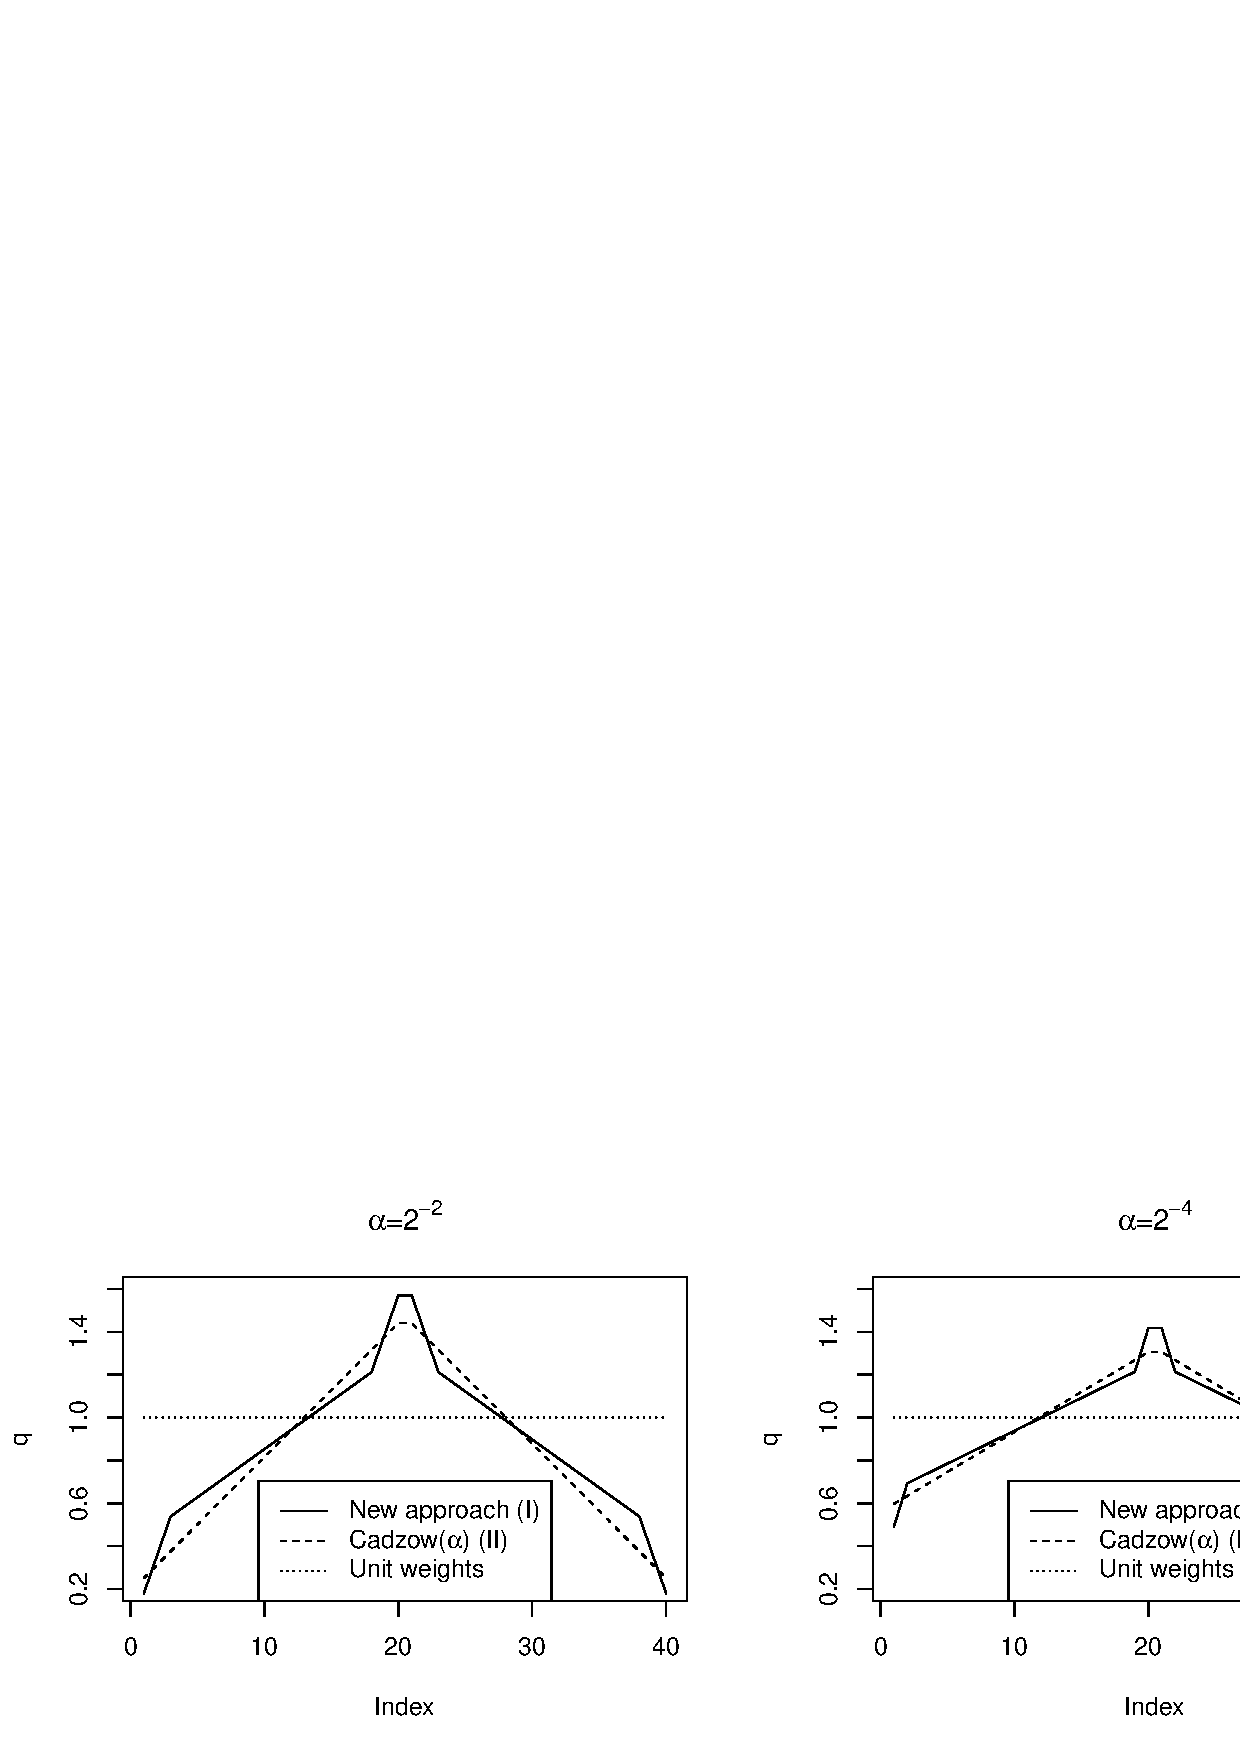
\includegraphics[width = \textwidth]{weights.pdf}\caption{Веса ряда}\label{img_weights}
\end{center}\end{figure}

\subsection{Комментарии к алгоритмам. Сравнение}

Итак, в дальнейшем будем рассматривать и сравнивать методы
Weighted Cadzow, Extended Cadzow, Cadzow ($\alpha$), $0< \alpha \leq 1$, совпадающий с обычным методом Cadzow при $\alpha=1$,
и Cadzow с $\widehat \bfC$.
Заметим, что длина окна $L$ является параметром всех рассматриваемых методов.

\begin{itemize}
\item
Все методы итеративные и, вообще говоря, они не обязаны сходится к глобальному экстремум в задаче МНК  (теоретически, даже сходимость можно иметь место только по подпоследовательностям; однако, во всех проведенных численных экспериментах сходимость имела место). Поэтому сравнение методов, даже
решающих одну и ту же задачу,  по точности имеет смысл.
\item
Сходимость методов по подпоследовательностям имеет место в предположении, что внутренние задачи проектирования в методах Weighted и Extended Cadzow решаются точно. Это напрямую следует из утверждения теоремы \ref{th:converg} для всех методов кроме Extended Cadzow, у которого веса являются частично нулевыми. Однако заметим, что  матрицы $\tilde \bfY_k$, которые содержат столбцы матриц $\Pi_{\calM_r} \bfY_k$ с $L$-го по $N$-ый и каждый элемент которых имеет положительный вес, являются матрицами ранга, не превосходящего $r$, их фробениусова норма не превосходит полунормы исходной матрицы: $\|\tilde \bfY_k\|_F \le \|\Pi_{\calM_r} \bfY_k\|_\bfM$, следовательно, эта ограниченная последовательность и у нее существует сходящаяся к нужному множеству подпоследовательность.
\item
Нас интересует сравнение методов не по достигаемому минимуму в задаче МНК, а по точности оценивания выделяемого сигнала $\bfS$.
Вполне возможно, что слишком хорошая аппроксимация исходного ряда может привести к переподгонке, результатом которой
может явиться ухудшение качества оценивания сигнала.
\item
Методы Weighted Cadzow и Extended Cadzow решают задачу \eqref{L-rank_task} c единичными весами $q_i$. Остальные методы решат задачу с весами, отличающимися от равных в той или иной степени.
\item
Однако каждая итерация методов Weighted Cadzow и Extended Cadzow отличается повышенной трудоемкостью, так как использует
еще один итеративный алгоритм на каждой основной итерации.
\item
Трудоемкость методов определяется как трудоемкостью одной итерации, так и числом итераций. Поэтому с этой точки зрения скорость сходимости представляет значительный интерес.
\item
На примере обычного метода Cadzow, известно, что при решении реальных задач одна итерация может представлять значительный интерес, как по трудоемкости, так и по широкому спектру решаемых задач. А именно, одна итерация метода Cadzow --- это известным метод Singular Spectrum Analysis (SSA), который умеет решать существенно большее число задач, чем сам итеративный метод. Поэтому представляет интерес также точность оценивания сигнала, выполненная с помощью одной итерации во всех рассматриваемых методах.
\item
В методе SSA есть понятие разделимости, которое определяет свойство метода (приближенно) находить сигнал по наблюдаемой сумме. Тем самым разделимость
тесно связана с точностью первой итерации итеративного метода. В свою очередь, естественно предположить, что точность первой итерации связана со скоростью сходимости метода. Поэтому вопросы разделимости имеют отношение к скорости сходимости итеративных алгоритмов.
\item
Связь разделимости с длиной окна $L$ для метода SSA хорошо изучена (см., например, \cite{Golyandina2010}). А именно, оптимальная длина окна близка
к половине длины ряда. Маленькие длины окна $L$ приводят к плохой разделимости. Влияние параметра $\alpha$ в классе алгоритмов
Cadzow ($\alpha$) на разделимость исследуется в приложении (раздел~\ref{sec:app}) на примере разделения константы и гармоники. Там показано, что малые значения
$\alpha$ приводят к плохой разделимости, хотя именно они соответствуют примерно равным весам $q_i$ в задаче \eqref{L-rank_task}.
В целом, виден следующий эффект: параметры, соответствующие более равномерным весам, приводят к худшей разделимости.
\item
Вполне возможно, что хорошая скорость сходимости и точность оценивания сигнала являются свойствами, которые не выполняются одновременно, как в силу
противоречия между равномерностью весов и разделимостью, так и потому что медленная сходимость вполне может привести к сходимости алгоритма к лучшему значению оптимизационной задачи.
\end{itemize}

\begin{remark}
\label{rem:adjust}
Во всех алгоритмах к $\widehat\tsS$ можно применить поправку \eqref{eq:adjust}, где $\|\cdot\|$ --- обычная евклидова норма независимо от алгоритма,
так как она согласуется с задачей \eqref{L-rank_task} с равными весами $q_i$.
Полученные алгоритмы будем называть алгоритмами с поправкой.
Например, результат работы $k$-й итерации алгоритма Cadzow можно записать как $\widehat\tsS_k = \calT^{-1}(\Pi_\calH \Pi_{\calM_r})^k \calT \tsX$.
Тогда результат $k$-й итерации алгоритма Cadzow с поправкой имеет вид $\widehat\tsS_k^*=\calA(\widehat\tsS_k)$.
\end{remark}

\section{Численные эксперименты}
\label{sec:simul}
В этом разделе мы приведем численные результаты, призванные продемонстрировать указанные выше выводы и соображения.
Сравнение было проведено для случая выделения синуса и экспоненциально-модулированного синуса.
Так как результаты, в целом, аналогичны, мы приведем только результаты, полученные для выделения гармонического ряда.

Был взят следующий сигнал:
\begin{equation*}
\tsS = (s_{1}, \ldots, s_N), \qquad s_{i} = 5\sin{\frac{2 \pi k}{6}}, \quad k = 1, \ldots, N, \quad N = 40
\end{equation*}
и рассматривался ряд в виде $\tsX = \tsS + \tsN$, где  $\tsN$ --- гауссовский белый шум с математическим ожиданием $0$ и дисперсией, равной $1$.
Точность оценивания сигнала оценивалась с помощью корня из среднего по точкам ряда и по 1000 реализациям ряда среднеквадратического отклонения (CKO)
$\widehat\tsS$ от сигнала $\tsS$.
Эту меру будем называть RMSE (root mean square error) оценки сигнала.
Сравнение проводилось на одних и тех же реализациях исходного ряда. Результаты сравнения являются значимыми
при уровне значимости 5\%.

Рассмотрим сначала класс методов Oblique Cadzow, включающий в себя и обычный метод Cadzow.
Рисунок \ref{img_cadzowspeed2} показывает одновременно скорость сходимости для разных значений параметра $\alpha$ и двух разных длин окна $L$.
По оси x откладывается номер итерации, по оси y --- RMSE оценки сигнала, деленное на число точек в ряде.
\begin{figure}[!hhh]
\begin{center}
\includegraphics[width = \textwidth]{cadzowspeed_2.pdf}
\caption{RMSE оценки сигнала в зависимости от числа итераций.}
\label{img_cadzowspeed2}
\end{center}
\end{figure}

В пределе самым лучших оказался самый медленно сходящийся метод, а именно, из рассмотренных методов это Cadzow (0.1) с длиной окна $L=8$.
Этот метод также соответствует наиболее равномерным весам из рассматриваемых в примере.
Заметим, что точность всех рассматриваемых методов различается не очень сильно, от 0.33 ($\alpha=0.1$, $L=8$) в лучшем случае до 0.37 в худшем
($\alpha=1$, $L=20$). Однако в первом случае ошибка 0.38 достигается уже на первой итерации, в то время как во втором для
достижения ошибки 0.38 требуется около 4--5 итераций.

Рассмотрим более подробно распределение ошибки по элементам ряда При этом включим в рассмотрение и
методы Extended и Weighted.
В качестве критерия остановки STOP1 для основных итераций будем использовать в алгоритмах число итераций, равное 100 (полученные результаты
можно считать предельными), а для внутренних итераций критерий STOP2 будет иметь вид $\frac{\|\bfY_k - \bfY_{k+1}\|^2}{LK} < 10^{-4}$.
Начальные левые и правые добавленные точки $\tsL_{L-1}$ и $\tsR_{L-1}$
в методе Extended Cadzow строились с помощью векторного SSA прогноза \cite[раздел 2.3.1]{Golyandina.etal2001}.

Возьмем длину окна $L=20$.  На рисунках~\ref{fig:s1_it1}~и~\ref{fig:s1_it100} по оси x откладывается номер точки ряда,
а по оси y --- RMSE от истинного значения сигнала в данной точке. Рисунок~\ref{fig:s1_it1} показывает ошибки на первой итерации,
а рисунок~\ref{fig:s1_it100} --- на итерации с номером 100.
Видно, что в обоих случаях самым точным оказывается метод Extended Cadzow. Из методов, не имеющих внутренних итераций,
на первой итерации выигрывают методы обычный Cadzow и Cadzow c $\widehat\bfC$. В пределе (после 100-й итерации результаты практически не меняются)
наилучшим из них, что не удивительно после анализа рисунка~\ref{img_cadzowspeed2}, оказался Cadzow с $\alpha=0.1$.

\begin{figure}[!hhh]
\begin{center}
\includegraphics[width = 13cm]{s1_it1.pdf}
\caption{RMSE оценки сигнала в каждой точке ряда на одной итерации.}
\label{fig:s1_it1}
\end{center}
\end{figure}

\begin{figure}[!hhh]
\begin{center}
\includegraphics[width = 13cm]{s1_it100.pdf}
\caption{RMSE оценки сигнала в каждой точке ряда на ста итерациях.}
\label{fig:s1_it100}
\end{center}
\end{figure}

Приведем таблицу~\ref{fintable}, где отражены результаты методов, а именно, RMSE как меры отклонения от сигнала и исходного ряда на одной и 100 итерациях.
В таблице $k$ --- число итераций, $\tsS$ --- сигнал, $\tsX$ --- исходный ряд; $L=20$. Таблица подтверждает выводы по сравнению методов по точности
оценивания сигнала. Также видно, что качество аппроксимации исходного ряда не всегда согласуется с качеством оценивания сигнала.
Например, для Cadzow c $\alpha=0.1$ на первой итерации явно видна переподгонка. Однако в пределе упорядоченность точности аппроксимации
и точности оценки сигнала одинаковые.

В таблице \ref{fintable_improved} содержатся аналогичные измерения для рядов с поправкой (см. замечание~\ref{rem:adjust}).
Видно, что поправка влияет незначительно (графики для результатов методов с поправкой мы не приводим, так как визуально влияние поправки незаметно). Аппроксимацию ряда поправка улучшает (не ухудшает) во всех случаях,
как и должно быть по ее построению. На точность оценивания сигнала поправка влияет неоднозначно. На 100-ой итерации она улучшает точность,
а на 1-й результаты разные.

\begin{table}[!hhh]
\begin{center}
\caption{Сравнение алгоритмов по RMSE.}\label{fintable}
\begin{tabular}{|c|c|c|c|c|}
\hline
$P$: & $\tsS$, $k = 1$ & $\tsX$, $k = 1$ & $\tsS$, $k = 100$ & $\tsX$, $k = 100$  \\
\hline
Cadzow, $\alpha = 1$ & 0.3758 & 0.9195 & 0.3782 & 0.9664 \\
\hline
Cadzow, $\alpha = 0.1$ & 0.4329 & 0.7040 & 0.3311 & 0.9506 \\
\hline
Cadzow $\hat{\bfC}$ & 0.3655 & 0.8925 & 0.3559 & 0.9583 \\
\hline
Weighted Cadzow & 0.3644 & 0.8891 & 0.3455 & 0.9549 \\
\hline
Extended Cadzow & 0.3361 & 0.9030 & 0.3189 & 0.9471 \\
\hline
\end{tabular}
\end{center}
\end{table}

\begin{table}[!hhh]
	\begin{center}
		\caption{Сравнение алгоритмов с поправкой по RMSE.}\label{fintable_improved}
		\begin{tabular}{|c|c|c|c|c|}
			\hline
			$P$: & $\tsS$, $T = 1$ & $\tsX$, $T = 1$ & $\tsS$, $T = 100$ & $\tsX$, $T = 100$  \\
			\hline
			Cadzow, $\alpha = 1$ & 0.3714 & 0.9175 & 0.3667 & 0.9622 \\
			\hline
			Cadzow, $\alpha = 0.1$ & 0.4385 & 0.7023 & 0.3276 & 0.9493 \\
			\hline
			Cadzow $\hat{\bfC}$ & 0.3626 & 0.8909 & 0.3478 & 0.9555 \\
			\hline
			Weighted Cadzow & 0.3640 & 0.8883 & 0.3380 & 0.9523 \\
			\hline
			Extended Cadzow & 0.3370 & 0.9030 & 0.3184 & 0.9469 \\
			\hline
		\end{tabular}
	\end{center}
\end{table}

\section{Заключение}
\label{sec:concl}
В работе были рассмотрены известные итеративные алгоритмы и предложены новые для аппроксимации ряда рядами конечного ранга с целью
оценивания сигнала в зашумленном ряде по взвешенному методу наименьших квадратов.


Был рассмотрен довольно широкий набор алгоритмов с целью получить равные веса в МНК. В рассматриваемых алгоритмах равные веса удалось
получить только с помощью вложенных итераций, которые сходятся только к локальному экстремуму и вдобавок делают алгоритм очень трудоемкими.
Итеративные методы без вложенных итераций дают только приближенно равные веса.

Для рассматриваемого класса алгоритмов типа алгоритмов Cadzow была доказана сходимость внешних итераций алгоритмов по подпоследовательностям.

На примере зашумленного синуса с помощью моделирования были получены результаты по точности и скорости сходимости предлагаемых алгоритмов.
Результаты показали, что самым точным оказывается самый трудоемкий метод.
Были рассмотрены вопросы соотношения скорости сходимости, трудоемкости и точности методов.
Акцент был сделан также на точности оценки с помощью одной итерации методов.

В дальнейшем предполагается провести расширенное численное и аналитическое исследование методов и получить более конкретные рекомендации по
соотношению трудоемкости и точности алгоритмов.

%\bibliographystyle{plain}
\bibliographystyle{gost2008}
\bibliography{zvonarev}
\addcontentsline{toc}{section}{Список литературы}

\section{Приложение: Разделимость константы и гармоники для двух алгоритмов Oblique Cadzow}
\label{sec:app}

Введем еще одну характеристику алгоритмов, показывающую, насколько хорошо они раскладывают временной ряд на его аддитивные компоненты. Основным применением описанных алгоритмов является задача оценки сигнала, поэтому данное качество нам важно для получения как можно более точной оценки.

Пусть $\bfC \in \sfR^{K \times K}$ --- симметричная неотрицательно определенная матрица, $\tsX_1$ и $\tsX_2$ ---  два разных временных ряда длины $N$, $\bfX^1$, $\bfX^2$ --- их траекторные матрицы. Тогда \emph{коэффициентом корреляции $i$-го и $j$-го столбца} назовем следующую величину:
\begin{equation}\label{col_corr}
\rho^c_{i,j} = \frac{(X^1_i, X^2_j)}{\|X^1_i\| \|X^2_j\|},
\end{equation}
где $X^k_i$ --- $i$-й столбец матрицы $\bfX^k$, $k = 1, 2$, $(\cdot, \cdot)$ --- евклидово скалярное произведение, $\|\cdot\|$ --- евклидова норма. \emph{Коэффициентом корреляции $i$-й и $j$-й строки} назовем следующую величину:
\begin{equation}\label{row_corr}
\rho^r_{i,j} = \frac{(X^{1,i}, X^{2,j})_\bfC}{\|X^{1,i}\|_\bfC \|X^{2,j}\|_\bfC},
\end{equation}
где $X^{k,i}$ --- $i$-я строчка матрицы $\bfX^k$, $k = 1, 2$, а $(\cdot, \cdot)_\bfC$ --- скалярное произведение с матрицей $\bfC$ в $\sfR^K$, определенная следующим образом: $(X, Y)_\bfC = X \bfC Y^\sfT$, так как $X$, $Y$ --- вектор-строчки, $\| \cdot \|_\bfC$ --- норма, порожденная этим скалярным произведением. Скажем, что ряды $\tsX_1$ и $\tsX_2$ \emph{слабо $\varepsilon$---разделимы}, если
\begin{equation}\label{weak_sep_eq}
\rho = \max\Big(\max_{1 \le i,j \le K}|\rho^c_{i,j}|, \max_{1 \le i,j \le L}|\rho^r_{i,j}|\Big) < \varepsilon.
\end{equation}
Нас будет интересовать порядок $\varepsilon$ при различных матрицах $\bfC$ и рядах $\tsX_1 = (c, c, \ldots)$ --- некоторая константа и $\tsX_2 = (\cos(2 \pi \omega k), k = 1, 2, \ldots)$, а также при различных $L$ и $K$ при условии, что мы будем брать только $N = L + K - 1$ компонент ряда. Когда $\bfC$ единичная матрица, ответ известен: $\varepsilon$ имеет порядок $1/\min(L,K)$, т.е. скорость сходимости имеет порядок $1/N$ при $L$, пропорциональном $N$.
Этот результат может быть найден в \cite[Раздел 6.1]{Golyandina.etal2001}. Он имеет отношение к точности первой итерации метода Cadzow.

В следующем утверждении рассматривается порядок разделимости для алгоритма Cadzow ($\alpha$), введенном в разделе~\ref{sec:cadzow_alpha}.

\begin{proposition}
\label{prop:separ1}
Пусть $\tsX_1 = (c, c, \ldots)$ --- некоторая константа и $\tsX_2 = (\cos(2 \pi \omega k), k = 1, 2, \ldots)$, где $0<\omega <0.5$, $L,K\ra \infty$ так, что $h = h_L = N/L$, где $N=L+K-1$, --- целое, и $\bfC$ определена в алгоритме Cadzow ($\alpha$), т.е.  $\bfC$ --- диагональная матрица со следующими диагональными элементами:
\begin{equation*}
c_k = \begin{cases}
1, & \text{если} \quad k = jL+1 \quad \text{для некоторого} \ j = 0, \ldots, h-1,\\
\alpha, & \text{в противном случае},
\end{cases}
\end{equation*}
где $0 \le \alpha \le 1$. Тогда $\rho$ имеет порядок $\max(\frac{1}{L}, \frac{(1-\alpha)C_{L,K}+\alpha}{(1-\alpha)N/L+\alpha K})$, где порядок $C_{L,K}$
может может меняться от $O(1)$ до $O(N/L)$ в зависимости от того, как $K$ стремятся к бесконечности.
\end{proposition}

\begin{proof5}{\ref{prop:separ1}}
Необходимо оценить порядки следующих величин:
\begin{gather*}
\rho^c_{i,j} = \frac{\sum_{k=j}^{j + L - 1} \cos(2 \pi \omega k)}{\sqrt{L (\sum_{k=j}^{j + L - 1} \cos^2(2 \pi \omega k))}},\\ \rho^r_{i,j} = \frac{\sum_{k=1}^K c_k\cos(2 \pi \omega (j + k - 1))}{\sqrt{(\sum_{k=1}^K c_k) (\sum_{k=1}^K c_k\cos^2(2 \pi \omega (j + k - 1)))}}.
\end{gather*}
Для доказательства используем следующие факты:
\begin{gather*}
\sum_{k=1}^n \cos(ak + b) = \csc(a/2) \sin(an / 2) \cos \left(\frac{an + a + 2b}{2} \right), \\
\sum_{k=1}^n \cos^2(ak + b) = \frac{1}{4}(\csc(a) \sin(2an + a + 2b) -\\ - \csc(a)\sin(a + 2b) + 2n),
\end{gather*}
для любых вещественных $a, b$ и положительного целого $n$.
Таким образом, когда ряд $\tsX_2$ не представляет из себя константу, числитель в $\rho^c_{i,j}$ имеет порядок $O(1)$, а знаменатель --- $O(L)$.
Первая часть доказана, и ее доказательство целиком аналогично случаю, когда $\bfC$ --- единичная матрица.

Для доказательства второй части выделим отдельно сумму по тем $k$, для которых $c_k=1$:
\begin{gather*}
\sum_{k=1}^K c_k\cos(2 \pi \omega (j + k - 1)) = (1-\alpha) \sum_{\substack{1 \le k \le K: \\ c_k = 1}}\cos(2 \pi \omega (j + k - 1)) +\\ +\sum_{1 \le k \le K}\alpha \cos(2 \pi \omega (j + k - 1)) = (1-\alpha) C_{L,K} + \alpha\, O(1),
\\
%\end{gather*}
%\begin{gather*}
\sum_{k=1}^K c_k = (1-\alpha) N/L + \alpha K,
\\
%\end{gather*}
%\begin{gather*}
\sum_{k=1}^K c_k\cos^2(2 \pi \omega (j + k - 1)) = (1-\alpha)\sum_{\substack{1 \le k \le K: \\ c_k = 1}}\cos^2(2 \pi \omega (j + k - 1)) +\\ +\sum_{1 \le k \le K }\alpha \cos^2(2 \pi \omega (j + k - 1)) = (1-\alpha) O(N/L) + \alpha\, O(K).
\end{gather*}
В худшем случае, если $L\omega$ целое, получаем, что $\cos(2 \pi \omega (j + k - 1))$ равно одной и той же константе независимо от $j$ и $k$, и тогда $C_{L,K}$ имеет порядок $O(N/L)$.
\end{proof5}

Таким образом, даже в лучшем случае, когда $C_{L,K}$ имеет порядок $O(1)$, разделимость константы и синуса становится хуже, чем при обычном варианте: при $\alpha$, близких к нулю, оптимальным выбором $L$ будет $L \approx \sqrt{N}$, и, таким образом, получаем порядок разделимости $1/\sqrt{N}$.

Теперь рассмотрим алгоритм Cadzow с $\widehat\bfC$, введенный в разделе~\ref{sec:cadzow_hat}.

\begin{proposition}
\label{prop:separ2}
Пусть $\tsX_1 = (c, c, \ldots)$ --- некоторая константа и $\tsX_2 = (\cos(2 \pi \omega k), k = 1, 2, \ldots)$, где $0<\omega <0.5$, $L,K\ra \infty$ и $\bfC$ определена в алгоритме Cadzow с $\widehat\bfC$.
 Тогда $\rho$ имеет порядок $\max \left(1/L, \frac{H_L}{\sqrt{NK}} \right)$ при $L, K \to \infty$, где $H_L$ --- $L$-е гармоническое число.
\end{proposition}

\begin{proof5}{\ref{prop:separ2}}
Необходимо оценить порядки следующих величин:
\begin{gather*}
\rho^c_{i,j} = \frac{\sum_{k=j}^{j + L - 1} \cos(2 \pi \omega k)}{\sqrt{L (\sum_{k=j}^{j + L - 1} \cos^2(2 \pi \omega k))}}, \\ \rho^r_{i,j} = \frac{\sum_{k=1}^K \hat c_k\cos(2 \pi \omega (j + k - 1))}{\sqrt{(\sum_{k=1}^K \hat c_k) (\sum_{k=1}^K \hat c_k\cos^2(2 \pi \omega (j + k - 1)))}}.
\end{gather*}
 Порядок $\rho^c_{i,j}$ уже был получен в доказательстве предложения~\ref{prop:separ1}, поэтому сразу перейдем к $\rho^r_{i,j}$. Рассмотрим корреляцию только первых строчек --- для остальных доказательство будет целиком аналогичным. Рассмотрим числитель $\rho^r_{1,1}$:
\begin{gather*}
\sum_{k=1}^K \hat c_k\cos(2 \pi \omega k) = \sum_{k=1}^{L-1} \hat c_k\cos(2 \pi \omega k) + \sum_{k=L}^{K - L + 1} \frac{\cos(2 \pi \omega k)}{L} +\\+ \sum_{k=K - L + 2}^{K} \hat c_k\cos(2 \pi \omega k) = I_1 + I_2 + I_3,
\end{gather*}
который разбился на три части. Для $I_2$ справедлива оценка $O(1/L)$, а для $I_3$ доказательство аналогично доказательству для $I_1$:
\begin{gather*}
|I_1|=\bigg|\sum_{k=1}^{L-1}\frac{1}{L}\left(\frac{k}{L} + \sum_{j=k}^{L-1} \frac{1}{j} \right) \cos(2 \pi \omega k)\bigg| =\\= \bigg|\sum_{k=1}^{L-1} \frac{k \cos(2 \pi \omega k)}{L^2} +  \frac{1}{L}\sum_{k = 1}^{L-1}\sum_{j = k}^{L-1}\frac{\cos(2 \pi \omega k)}{j}\bigg| \le \\ \le
\bigg|\sum_{k=1}^{L-1} \frac{k \cos(2 \pi \omega k)}{L^2}\bigg| + \bigg|\frac{1}{L}\sum_{k = 1}^{L-1}\sum_{j = k}^{L-1}\frac{\cos(2 \pi \omega k)}{j}\bigg|.
\end{gather*}
Используя тот факт, что
\begin{gather*}
\sum_{k=1}^n k \cos(ak + b) = -\frac{1}{4}\csc^2(a/2)(-(n+1)\cos(an+b) + \\ + n\cos(an + a + b) + \cos b),
\end{gather*}
получаем:
\begin{gather*}
\bigg|\sum_{k=1}^{L-1} \frac{k \cos(2 \pi \omega k)}{L^2}\bigg| = O(1/L), \quad
\bigg|\frac{1}{L}\sum_{k = 1}^{L-1}\sum_{j = k}^{L-1}\frac{\cos(2 \pi \omega k)}{j}\bigg| = \\ =\bigg|\frac{1}{L}\sum_{j = 1}^{L-1}\sum_{k = 1}^{j}\frac{\cos(2 \pi \omega k)}{j}\bigg| \le \bigg|\frac{1}{L}\sum_{j = 1}^{L-1}\frac{d}{j}\bigg| = O \left(\frac{H_L}{L} \right),
\end{gather*}
где $d$ --- некоторая константа. 

Для знаменателя нужно рассмотреть следующие суммы:
\begin{equation*}
\sum_{k=1}^K \hat c_k = N / L
\end{equation*}
по определению, а следующую составляющую просто оценить снизу:
\begin{equation*}
\sum_{k=1}^K \hat c_k\cos^2(2 \pi \omega (j + k - 1)) \ge \sum_{k=1}^K \frac{1}{L}\cos^2(2 \pi \omega (j + k - 1)) = O \left(\frac{K}{L} \right).
\end{equation*}
\end{proof5}


\end{document}
